%\documentclass[paper]{geophysics}
\documentclass[manuscript,revised]{geophysics}


\usepackage{setspace}
\usepackage[colorlinks]{hyperref}
\hypersetup{colorlinks=true,linkcolor={blue},citecolor={blue},urlcolor={red}} 

\usepackage{amsmath}
\usepackage[utf8x]{inputenc}
\usepackage{graphicx}
\graphicspath{ {./images/} } % images path

\usepackage{multirow} % for tables
\usepackage[table,xcdraw]{xcolor}
\usepackage{floatrow} % for caption on the top of the table

\usepackage[nameinlink, capitalise, noabbrev]{cleveref} % enhance refs

\usepackage[document]{ragged2e} % to justify text

%\usepackage{ragged2e}
\DeclareCaptionJustification{justified}{\justifying} 			% to justify figure caption
%\captionsetup{compatibility=false,justification=justified} 		% to justify figure caption
%\DeclareCaptionFormat{custom}{\textbf{#1#2}\textit{\small #3}}
\DeclareCaptionFormat{custom}{\textbf{#1#2}{\small #3}}
\captionsetup{compatibility=false, justification=justified, format=custom}

% An example of defining macros
\newcommand{\rs}[1]{\mathstrut\mbox{\scriptsize\rm #1}}
\newcommand{\rr}[1]{\mbox{\rm #1}}

% found it here: https://stackoverflow.com/questions/70705684/latex-get-figure-caption-to-align-with-image
%%%%%%%%%%%%%%%%%%%%%%%%%%%%%%%%%%%%%%%%%%%%%%%%%%%%
\usepackage{blindtext} % Package to generate dummy text throughout this template 
\usepackage[sc]{mathpazo} % Use the Palatino font
\usepackage[T1]{fontenc} % Use 8-bit encoding that has 256 glyphs
\linespread{1.05} % Line spacing - Palatino needs more space between lines
\usepackage{microtype} % Slightly tweak font spacing for aesthetics
\usepackage[english]{babel} % Language hyphenation and typographical rules

\usepackage[hmarginratio=1:1,top=32mm,columnsep=20pt]{geometry} % Document margins
\usepackage{lettrine} % The lettrine is the first enlarged letter at the beginning of the text

\usepackage{enumitem} % Customized lists
\setlist[itemize]{noitemsep} % Make itemize lists more compact

\usepackage{fancyhdr} % Headers and footers
\pagestyle{fancy} % All pages have headers and footers
\fancyhead{} % Blank out the default header
\fancyfoot{} % Blank out the default footer
\fancyhead[L]{Manuscript} % Custom header text
\fancyfoot[RO,LE]{\thepage} % Custom footer text


\setlength\parindent{24pt}
%\usepackage{float}
\usepackage{floatrow}
\usepackage{pdfpages}
\newsavebox\mysavebox


\usepackage{booktabs} % to import tables directly from python
%%%%%%%%%%%%%%%%%%%%%%%%%%%%%%%%%%%%%%%%%%%%%%%%%%%



\begin{document}

\title{?????????????????}
\renewcommand{\thefootnote}{\fnsymbol{footnote}} 
\ms{GEO-Example} % manuscript number

\address{
\footnotemark[1]BP UTG, \\
200 Westlake Park Blvd, \\
Houston, TX, 77079 \\
\footnotemark[2]Bureau of Economic Geology, \\
John A. and Katherine G. Jackson School of Geosciences \\
The University of Texas at Austin \\
University Station, Box X \\
Austin, TX 78713-8924}

\author{Gelson Ferreira de Souza-Junior\footnotemark[1], Ricardo Ivan Ferreira da Trindade\footnotemark[1],  Leonardo Uieda\footnotemark[2]}
\date{June 2022}
\footer{Example}
\lefthead{Dellinger \& Fomel}
\righthead{\emph{Geophysics} example}

\maketitle
\justify

\begin{abstract}
\begin{singlespace}
Paleomagnetism is the main tool used in paleogeographic reconstructions, in which directional information of the past magnetic field is retrieved from ferromagnetic grains (l.s). Magnetic minerals have a wide range of size and composition that influence their magnetic properties and, consequently, their ability to record the directions of paleomagnetic fields. The signals obtained with classical paleomagnetic methodologies are vector averages that include all magnetic grains present in the samples, including the stable and unstable carriers. To improve the quality of the magnetic signal, it would be necessary to individually identify the magnetizations of the carriers of remanent magnetization, in order to isolate only the good registers of the geomagnetic field. This would allow obtaining more reliable paleomagnetic information, as well as possibly being effective for the paleomagnetic study of older rocks (e.g., Archean rocks), meteorites and even bodies with complex geological evolution. Therefore, this project aims to apply magnetic microscopy to identify the remanent magnetization directions of stable magnetic grains and, subsequently, invert these data in an attempt to recover the individual paleomagnetic directions of the magnetic carriers present in the thin-sections. If successful, a new precision methodology for paleomagnetic data acquisition will be implemented.

\noindent{\textbf{Keywords}: Paleomagnetism, magnetic microscopy, Euler deconvolution, inversion of magnetic data.}
\end{singlespace}
\end{abstract}


\begin{singlespace}

\section{Introduction}
%\onehalfspacing
%\doublespacing

\noindent{Paleomagnetism is the study of the record of the Earth's magnetic field preserved in rocks, being the main tool, and the only quantitative method, used during paleogeographic reconstruction~\citep{Butler1992}. It is based on three basic assumptions: (i) the geomagnetic field can be approximated to the field created by a geocentric axial dipole (GAD) aligned with the Earth's axis of rotation over a period that eliminates paleosecular variation ($>10^4$ years)~\citep{McElhinny2000}; (ii) ferromagnetic minerals (l.s.) acquire natural remanent magnetization (NRM) parallel to the Earth's geomagnetic field~\citep{Dunlop1997, Tauxe2018}; and (iii) this acquired magnetization is recorded for a long period of time, depending on the physicochemical characteristics of the magnetized mineral, following Neél's Theory~\citep{Neel1949, Neel1955} and being also influenced by the geological processes by which the rocks were submitted.}

\noindent{The thermoremanent magnetizations (TRMs) of magnetic particles in geological materials are the main records of the direction of the geomagnetic field of the past \citep{DeGroot2014}. Iron oxides, such as magnetite, which is the most common magnetic mineral present in rocks~\citep{OReilly1984} and acquire TRM as they cool below their Curie temperature and subsequently this direction of magnetization is “frozen” upon reaching blocking temperature~\citep{Dunlop1997}. When the grains are small enough, and the magnetization is unidirectional homogeneous (single domain - SD), the acquisition and preservation of magnetic signals is physically supported by Néel's theory~\citep{Neel1949, Neel1955}, conserving the remanent magnetization for long periods of time, on the order of billions of years, and for this reason, they are considered “good recorders” of the paleomagnetic field. In addition to SD, pseudo-single domain (PSD) particles, in the flower and stable vortex states, can also preserve magnetization for periods on the order of the solar system age~\citep{Nagy2017}. On the other hand, Néel's theory does not cover larger particles (multi domain - MD), which have unstable remanent magnetization (e.g., caused by viscous reordering of magnetic domains,~\cite{DeGroot2014}), so they are particles with limited ability to record the geomagnetic field. In addition to the magnetic domain state, particles can still vary in composition, size and shape which causes changes in their magnetic properties. All these factors are crucial in determining stable remanence directions used in the calculation of paleomagnetic poles.}

\noindent{Classic techniques for obtaining paleomagnetic data, e.g., thermal demagnetization and alternating fields, are based on the progressive acquisition of the magnetization contained in cylindrical samples, usually of 10 cm$^3$. The magnetic signal of a single specimen is the result of the sum of moments contained in the assembly of ferromagnetic grains, including stable and unstable registers~\citep{DeGroot2021}. Although there are recent well-structured studies of imaging magnetic minerals in thin-sections \citep[e.g.,][]{Almeida2014, Farchi2017,  Glenn2017, Lima2014, Lima2009, Nichols2016, Weiss2007, DeGroot2018, DeGroot2021}, obtaining NRM directions of individual grains in the rock fabric remains, to the best of our knowledge, a challenge deeply explored only by \cite{DeGroot2021}. With the possibility of isolating the individual contributions of a fairly large number ($10^6$ $>$ N $>$ $10^7$) of stable magnetic particles (SD/PSD) the magnetic directions recovered, using the average of their NRM vectors, would have an accurate paleomagnetic response \citep{Berndt2016}, however such number of observations is unfeasible for the currently insufficient measurements scales of the equipaments \citep{DeGroot2018}.}

\noindent{Several branches of Earth Sciences have demonstrated the importance of the “spatiality" of data on a microscopic scale, mainly in Geochemistry and Geochronology, where it is possible to perform punctual analyzes and compositional maps, which allowed significant advances in the understanding of igneous, metamorphic and sedimentary processes~\citep[e.g.,][]{ Barnes2019, Davidson2007, Verberne2020}. In Paleomagnetism there has been an interest in point magnetic analyses, or microscale magnetic maps, from magnetic microscopy techniques~\citep{DeGroot2014, DeGroot2018, Lima2014, Weiss2007}. However, despite recent advances in this area, still there is no well-established inversion protocol to determine the magnetic vector direction of each individual ferromagnetic grains, nor the intensity of magnetization, without using additional information of the positioning and shape of these sources, such as micromagnetic tomography \citep[e.g.,][]{DeGroot2018, DeGroot2021, Fabian2019}, which is a measurement spatially even more limited than the magnetic microscopy itself.}

\noindent{This paper aims to give a new perspective in the methodological routine that carry out paleomagnetic studies in microscale allowing to retrieve the individual remanent magnetization direction of these stable magnetic carriers (SD and PSD), semi automatically and without any additional information. In this way, a larger area of the thin section can be scanned with the objective of increasing the number of observations and, therefore, increasing the reliability of the directional data obtained. We also intend to generate a micromagnetic analysis protocol in an open source software, based on the techniques that will be described below.}

%%%%%%%%%%%%%



\end{singlespace}

\section{Methodology}
%%%
\subsection{Scanning Magnetic Microscopy}

\noindent{Scanning magnetic microscopy (SMM) is the imaging technique in which a thin-section sample of geological material is horizontally displaced under a high-precision (fixed) micromagnetometer to obtain magnetization \citep{Weiss2007}. The SMM performed at a fixed height above the sample also has the advantage of facilitating the subtraction of the ambient field (constant), to which it might be subject during the scan \citep{Lima2013}. The availability of high-performance and low-cost magnetic sensors has promoted a great advance in the application of SMM in recent years. However, its sensitivity is still a few orders of magnitude lower than that of superconducting quantum interference devices (SQUIDs), the latter being between 10$^{-12}$ and 10$^{-15}$ Am$^2$ \citep{Lima2013}. This disadvantage is offset by (i) the high spatial resolution of the SMM, as it is performed at a few tens of micrometers from the sampled surface; and (ii) SQUID magnetic microscopy is performed at low temperatures ($<$ 100K), which can cause changes in the original NRM of the sample, while SMM is performed at room temperature \citep{Lima2013, Weiss2007}.}

\noindent{The SMM can also be considered as a form of aeromagnetic survey, carried out at microscales on sources of flat topography, with high spatial resolution and greater sensitivity to magnetic moment \citep{Lima2013}. An emerging magnetic imaging technology is the quantum diamond microscope (QDM) with very high spatial resolution ($≅$ 1 μm), and can recover magnetic moments as weak as 10$^{-17}$ Am$^2$, through magnetic sensors located at altitudes between 1 and 5 µm relative to the sample surface \citep{Fu2020} capable of detecting the magnetic signals of SD magnetite particles (\cref{fig:QDM}). Another promising type of magnetic microscope is the magnetic tunnel junction (MTJ) with a spatial resolution greater than 7 µm, a magnetic moment sensitivity of up to 10$^{-14}$ Am$^2$ and sample-sensor distance of 7 µm. Its advantages reside in the fact that these MTJ devices do not require high bias current to operate (few tens of µA), which avoids induced magnetization signals created by artificial magnetic field during the measurements \citep{Lima2014}.}

\begin{figure}[htbp]
\centering
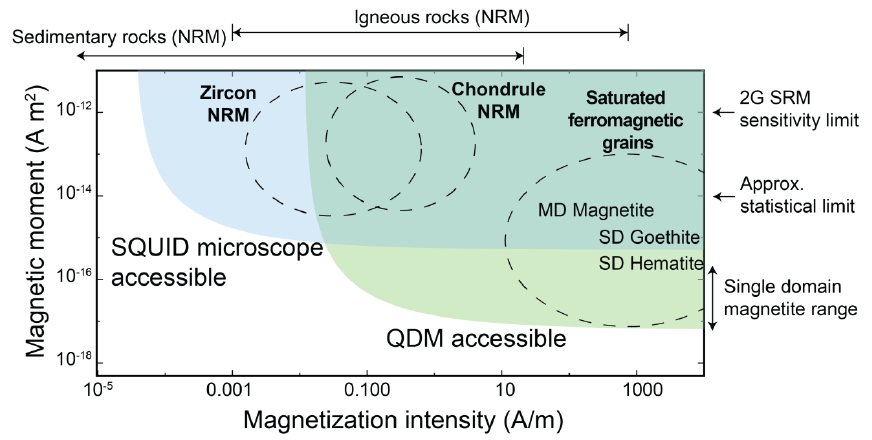
\includegraphics[width=\textwidth]{QDM.png}
\caption{Sample classes accessible to QDM, SQUID microscope and 2G Enterprises SRM. The accessible region for the QDM was calculated assuming a magnetic field noise threshold of 5 nT and a minimum sensor-sample distance of 5 μm. The calculation for the SQUID microscope assumed field noise values of 15 pT and sensor-sample distance of 150 μm. Source: \cite{Fu2020}.}
\label{fig:QDM}
\end{figure}

\noindent{Due to the similarities between magnetic microscopy techniques and aeromagnetic surveys, the methodologies of data inversion of the latter, densely studied in the last decades, can be adapted for magnetic microscopy. However, \cite{Lima2013} report important distinctions between SMM and aeromagnetic surveys, namely: (i) the source distribution in the SMM can often be accurately modeled in a two-dimensional model; (ii) the SMM measures the field produced directly by the sample's NRM; (iii) the sensor positioning is very accurate in the SMM, and the vertical component of the magnetic field is usually measured, rather than the total field; (iv) there is no need for correction to bring all measurements to the same surface or to grid the data; and (v) the distributions of the magnetization sources are finite and known.}




%%%
\subsection{Euler Deconvolution}

\noindent{\cite{Thompson1982} proposed the Euler Deconvolution technique, which is a consolidated method classically applied to data from aeromagnetic surveys that uses first order x, y and z derivatives to determine the positioning and depth of ideal targets (e.g., sphere, cylinder), each characterized by a structural index \citep{Nabighian2005}. Euler deconvolution is one of the most useful methods for estimating the three-dimensional positioning of magnetic sources/geological bodies \citep{Reid1990}. Given the similarities between SMM and aeromagnetic data, its application becomes plausible for determining the positions of magnetic sources caused by ferromagnetic minerals (l.s).} 

\noindent{The classic Euler approach is basically the application of a mobile operator in a small data window over the sampled dataset. The observations made within this window are used to estimate the horizontal and vertical positions of the source by solving a small linear system of equations using the gradients of the potential field, provided that the shapes of the sources are assumed. Despite this, this methodology usually yields a large number of solutions \citep{Barbosa2011}, which becomes a limitation for the method. In an attempt to circumvent the problem of this expressive cloud of solutions, we suggest a previous application of a method for delimitating the region of each source that generates the potential field and later the application of Euler's Deconvolution. Hence giving a single system of linear equations to be solved for each source.}

\noindent{Derivative-based filters are widely used to emphisize the potencial anomaly signal of shallower sources and applied in modern methods for edge/position detection, as of the solution of Euler equation itself requires the gradient of the potential field. Since the calculation of first order derivatives is a must in this case, we might as well give preference to filtering techniques that use the same products. One good filtering example is the so called horizontal gradient method ($\nabla H$, \cref{eq:HG}) \citep{Cordell1982}, which is a source edge detection methodology where the response of a target's horizontal gradient tends to overlap its own limits, thus obtaining a two-dimensional robust map of the sources location \cite{Blakely1996}. Another popular method for locating edges of magnetic bodies is the total gradient ($\nabla T$, \cref{eq:TG}), which places the source's maximum anomaly values over the area inside its boundaries, despite of  geomagnetic latitude, magnetization direction or source dip/geometry \citep{Nabighian2005}. Both total and horizontal gradients are reliable techniques to be applied with the SMM data.}


\begin{equation} \label{eq:HG}
\centering
\nabla H= \sqrt{ {\left( \frac{∂F}{∂x} \right)}^2+{\left( \frac{∂F}{∂y} \right)}^2 }
\end{equation}

\begin{equation} \label{eq:TG}
\centering
\nabla T= \sqrt{ {\left( \frac{∂F}{∂x} \right)}^2+{\left( \frac{∂F}{∂y} \right)}^2+{\left( \frac{∂F}{∂z} \right)}^2 }
\end{equation}


\noindent{After pre processing the data with derivative-based filter, highlighting the sources edges, it is possible to apply blob detection techniques. The latter refers to visual algorithms and/or modules with the ability of detecting points/regions that are either darker or brighter than the neighborhood. The most common and accurate approach to detect brighter blobs on dark surroundings is the Laplacian of Gaussian (LoG), its downside is also being slower than other approaches \citep{Han2016, Kong2013}. We used the \href{https://scikit-image.org/docs/stable/auto_examples/features_detection/plot_blob.html#sphx-glr-auto-examples-features-detection-plot-blob-py}{scikit-image blob detection} python library \citep{VanderWalt2014} to identify the window region of data that embraces each isolated source by applying the algorithm on the highlighted sources map ($\nabla T$ or $\nabla H$). Therefore, the blobs selected are local maxima obtained with successively LoG images. Once the target location window is determined, subsequently, the Euler Deconvolution can applied in this single static data window yeilding only one solution per source. Thus, being an automatic, faster and easier way than the classical methodology of solving the Euler equation.}


%%%
\subsubsection{Euler Deconvolution Formulation}

\noindent{The anomaly of a potential field F produced by a three-dimensional source, whose cartesian coordinates of its central position are x$_c$, y$_c$ and z$_c$, satisfies the homogeneous Euler equation \citep{Reid1990} expressed by:}

\begin{equation} \label{eq:euler1}
\centering
(x-x_c) \cdot \frac{\partial F}{\partial x} + (y-y_c) \cdot \frac{\partial F}{\partial y}+(z-z_c) \cdot \frac{\partial F}{\partial z}=n \cdot (b-F)  \ \ 
\end{equation}

\begin{tabular}{ l }
\noindent{where: n is the structural index, that is, a gauge of the geometric shape of the}  \\
\noindent{sources causing the anomaly; and b is the constant, and unknown, base level.}  \\
\end{tabular}

\bigskip

\noindent{The Euler's Deconvolution uses the gradient of a potential field and the structural index, which can be defined by the geometric nature of the sources. The structural index is the only necessary a priori knowledge. Once a value for n is assumed (n = 3 for spherical/punctual magnetic sources), the homogeneous Euler equation can be rearranged as follows:}

\begin{equation} \label{eq:euler2}
\centering
x_c \cdot \frac{\partial F}{\partial x} + y_c \cdot \frac{\partial F}{\partial y} + z_c \cdot \frac{\partial F}{\partial z} + n \cdot b = x \cdot \frac{\partial F}{\partial x} + y \cdot \frac{\partial F}{\partial y} + z \cdot \frac{\partial F}{\partial z} + n \cdot F  \ \ 
\end{equation}

\noindent{The \cref{eq:euler2} can be written in matrix form as:}

\begin{equation} \label{eq:euler3}
\centering
\left[\begin{matrix}{Fx}_1&{Fy}_1&{Fz}_1&n\\{Fx}_2&{Fy}_2&{Fz}_2&n\\\vdots&\vdots&\vdots&\vdots\\{Fx}_N&{Fy}_N&{Fz}_N&n\\\end{matrix}\right]\left[\begin{matrix}x_c\\y_c\\z_c\\b\\\end{matrix}\right]=\left[\begin{matrix}x_1\cdot{Fx}_1+y_1 \cdot {Fy}_1+z_1 \cdot {Fz}_1+n\cdot F_1\\x_2\cdot{Fx}_2+y_2\cdot{Fy}_2+z_2\cdot{Fz}_2+n\cdot F_2\\\vdots\\x_N\cdot{Fx}_N+y_N\cdot{Fy}_N+z_N\cdot{Fz}_N+n\cdot F_N\\\end{matrix}\right]\ 
\end{equation}

\begin{tabular}{ l }
\noindent{Where: $Fx_i$, $Fy_i$ and $Fz_i$ represent, respectively, the gradients $\frac{\partial F}{\partial x}$, $\frac{\partial F}{\partial y}$ and $\frac{\partial F}{\partial z}$}   \\
\noindent{evaluated on the i-th observation point ($i=1,2, ..., N$). While $x_i$, $y_i$ and $z_i$}   \\
\noindent{represent the cartesian coordinates at the i-th observation point.}
\end{tabular}

\bigskip

\noindent{Note that \cref{eq:euler3} is a linear system $\bar{\bar{G}} \cdot \bar{p}=\bar{d}$ and its objective function $f(\bar{p} )$ expressed by:}

\begin{equation} \label{eq:euler4}
\centering
f(\bar{p} ) = {\lVert e\lVert}^2 = {(\bar{\bar{G}} \cdot \bar{p}-\bar{d})}^T \cdot ~ (\bar{\bar{G}} \cdot \bar{p}-\bar{d})
\end{equation}

\noindent{The solution $\bar{p}$ of the system can be obtained by minimizing the objective function $(\frac{\partial f}{\partial p_k}=\bar{0})$ through the least squares estimator given by:}

\begin{equation} \label{eq:euler5}
\centering
\bar{p}=\left({\bar{\bar{G}}}^T\cdot ~ \bar{\bar{G}}\right)^{-1} \cdot \ \left({\bar{\bar{G}}}^T\cdot ~ \bar{d}\right)
\end{equation}

\noindent{Thus, $\bar{p}=\left[x_c\ \ y_c\ \ z_c\ \ b\right]^T$ will be the solution vector that satisfies Euler's Equation with the least possible error containing the position coordinates source center ($x_c$, $y_c$, $z_c$) and the base level (b).}









%%%
\subsection{Magnetic Inversion}

\noindent{The rapid inversion of the total field is a method developed by \cite{OliveiraJr.2015} being computationally efficient to invert the magnetic anomalies produced by multiple sources with approximately spherical shapes to estimate their magnetization directions (inclination and declination). This methodology requires the central position of the magnetic sources, which can be obtained with Euler Deconvolution, and the information on their geometry helps to reduce the non-exclusivity of the problem. In this way, it is possible to estimate the direction of magnetization from multiple sources. The method does not require that all sources have the same magnetization direction nor the use of regularly spaced data on a horizontal grid, and can still be implemented in linear and non-linear inversion problems.}

\noindent{Currently, the main inversion limitations for these type of data are: (i) in part because the sampling scale during measurement is insufficiently accurate and (ii) because of the non-singularity of the magnetic inversion  \citep{Lima2013}. The basic mathematical structure associated with the inverse problem of aeromagnetic data can be adapted and used in SMM data due to its similarity, despite the non-singularity caused by the infinite number of solutions for the same observed magnetic field  \citep{Weiss2007}. Assigning as much information as possible about the analyzed sample and the experimental environment can reduce this ambiguity by recovering the magnetization direction. In particles with unidirectional magnetization, and without magnetization sources outside the sample area, it is possible to guarantee singularity for the inverse problem in SMM  \citep{Baratchart2013}. Associating the fact that there is a singularity in the response of uniformly magnetized particles and that ferromagnetic particles (\emph{l.s.}) with stable magnetization have such a characteristic, therefore, the inversion method becomes ideal for the purpose of this project.}

%%
\subsubsection{Parametrization and Forward Model}

\noindent{Let $\bar{B}$ be the observed data vector, whose i-th element ${\bar{B}}_i$, $i= 1, 2, ..., N$, is a total field anomaly, resulting from the NRM contribution of each ferromagnetic particle (\emph{l.s.}), measured at position ($x_i$, $y_i$, $z_i$) (black dots, \cref{fig:model_plus_vector}a). In this cartesian coordinate system, x points to geographic north, y points east, and z points down. In general, the magnetic field that is produced in the thin section is the result solely and exclusively of the NRM contribution of the particles without considering the induced component, since the measurements carried out in the magnetic microscope are usually made under magnetic shielding conditions. Thereby, approximating the shape of ferromagnetic minerals (\emph{l.s.}) to NRM magnetizing spheric/punctual sources. According to \cite{Blakely1996} the equation of a uniformly magnetized sphere is given by:}

\begin{equation} \label{eq:sphere1}
\centering
b =\ C_m \cdot \frac{4}{3} \cdot \pi \cdot R^3 \cdot M \cdot \hat{M} \cdot \frac{1}{r^2} \cdot \hat{r}
\end{equation}

\noindent{Whereas the magnetic sources can be represented by a set of L uniformly magnetized spheres. In this case, each sphere will have a contribution in the field measured at the position ($x_i$, $y_i$, $z_i$):}

\begin{equation} \label{eq:sphere2}
\centering
{b_i}^j=\ C_m \cdot \frac{4}{3}\pi \cdot {R_j}^3 \cdot {\bar{M}}^j\cdot\frac{1}{r_{i,j}^2}\cdot{\hat{r}}_{i,j}\ ,\ \ j=1,\ 2\ldots,\ L
\end{equation}

\begin{tabular}{ l }
\noindent{Where: $C_m=\ \frac{\mu_0}{4\pi}=\ {10}^{-7}\frac{\ H}{m}$; $R_j$ is the radius of the j-th sphere; $r_{i,j}$ is the distance}   \\ 
\noindent{(unit vector ${\hat{r}}_{i,j}$) between the center of the j-th sphere and the observation point i,}    \\  
\noindent{i = 1, 2, . .. N; and ${\bar{M}}^j=\left[{Mx}_j\ {My}_j\ {Mz}_j\right]^T$ is the vector formed by the cartesian} \\
\noindent{components of the magnetization of the j-th sphere (unit vector ${\hat{M}}^j)$.}
\end{tabular}

\bigskip

\begin{figure}[htbp]
\centering
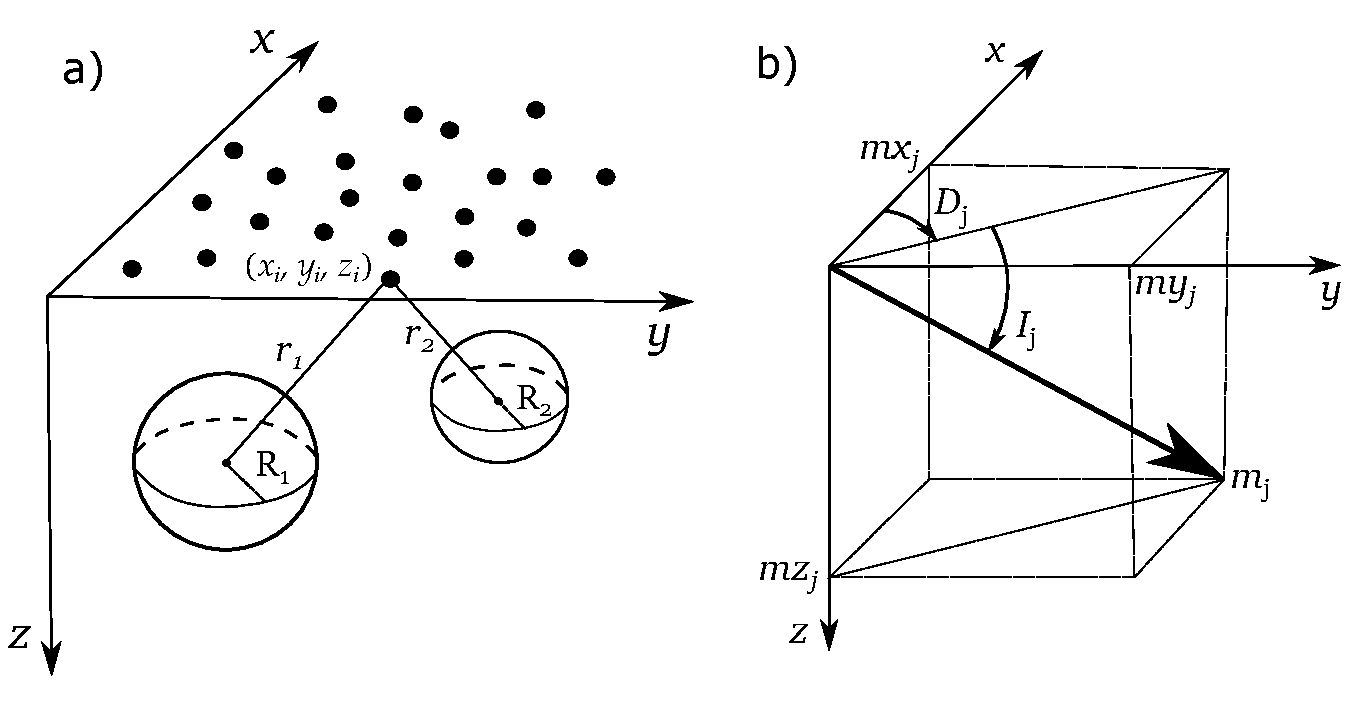
\includegraphics[width=0.8\textwidth]{model_plus_vector.pdf}
\caption{a) Schematic representation of spheres (L = 2) uniformly magnetized in the subsurface, whose magnetic effect can be observed at points ($x_i$, $ y_i$, $z_i$), i = 1, 2, ..., N (black dots). In this cartesian coordinate system x, y and z corresponds to geographic north, east and z, respectively. b) Schematic cartesian representation of vector $m_j$ with elements $mx_j$, $my_j$ and $mz_j$, with declination $D_j$ (positive clockwise) and inclination $I_j$ (positive downwards), j = 1, 2, ... L. Modified from: \cite{OliveiraJr.2015}.}
\label{fig:model_plus_vector}
\end{figure}

\noindent{Thus, the total magnetization measured at the position ($x_i$, $y_i$, $z_i$) will be the sum of contributions from the L spheres, given by:}

\begin{equation} \label{eq:sphere3}
\centering
B_i=\sum_{j=1}^{L}b_i^j
\end{equation}

\noindent{The \cref{eq:sphere2} presents the sensitive matrix $A_i^j$ and the $m_j$, which is the vector that encompasses the cartesian components of the magnetc moment (magnetization times volume) of each sphere:}

\begin{equation} \label{eq:sphere4}
\small A_i^j ={C}_{m} \cdot \left[\begin{matrix}\left(\frac{\partial^2}{\partial x\partial x}\cdot\frac{1}{r_{i,j}}\right)&\left(\frac{\partial^2}{\partial x\partial y}\cdot\frac{1}{r_{i,j}}\right)&\left(\frac{\partial^2}{\partial x\partial z}\cdot\frac{1}{r_{i,j}}\right)\\\left(\frac{\partial^2}{\partial x\partial y}\cdot\frac{1}{r_{i,j}}\right)&\left(\frac{\partial^2}{\partial y\partial y}\cdot\frac{1}{r_{i,j}}\right)&\left(\frac{\partial^2}{\partial x\partial z}\cdot\frac{1}{r_{i,j}}\right)\\\left(\frac{\partial^2}{\partial x\partial z}\cdot\frac{1}{r_{i,j}}\right)&\left(\frac{\partial^2}{\partial y\partial z}\cdot\frac{1}{r_{i,j}}\right)&\left(\frac{\partial^2}{\partial z\partial z}\cdot\frac{1}{r_{i,j}}\right)\\\end{matrix}\right]_{\text{\tiny 3N $\times$ 3L}},
m_j =\left[\begin{matrix}{{Mx}_{j\ }} \cdot \frac{4}{3}\pi\cdot R_j^3\\{{My}_{j\ }} \cdot \frac{4}{3}\pi\cdot R_j^3\\{{Mz}_{j\ }} \cdot \frac{4}{3}\pi\cdot R_j^3\\\end{matrix}\right]_{\text{\tiny 3L $\times$ 1}}
\end{equation}

\begin{FlushRight}
\noindent{Where: $\frac{1}{r_j}\equiv\frac{1}{\sqrt{\left(x_i-{xc}_j\right)^2+\left(y_i-{yc}_j\right)^2+\left(z_i-{zc}_j\right)^2}}$}
\end{FlushRight}

\noindent{Subsequently, the components of the total magnetizing field can be obtained (from \cref{eq:sphere3}), as shown below:}

\begin{equation} \label{eq:sphere5}
\small {C}_{m} \cdot \left[\begin{matrix}\left(\frac{\partial^2}{\partial x\partial x}\cdot\frac{1}{r_{i,j}}\right)&\left(\frac{\partial^2}{\partial x\partial y}\cdot\frac{1}{r_{i,j}}\right)&\left(\frac{\partial^2}{\partial x\partial z}\cdot\frac{1}{r_{i,j}}\right)\\\left(\frac{\partial^2}{\partial x\partial y}\cdot\frac{1}{r_{i,j}}\right)&\left(\frac{\partial^2}{\partial y\partial y}\cdot\frac{1}{r_{i,j}}\right)&\left(\frac{\partial^2}{\partial x\partial z}\cdot\frac{1}{r_{i,j}}\right)\\\left(\frac{\partial^2}{\partial x\partial z}\cdot\frac{1}{r_{i,j}}\right)&\left(\frac{\partial^2}{\partial y\partial z}\cdot\frac{1}{r_{i,j}}\right)&\left(\frac{\partial^2}{\partial z\partial z}\cdot\frac{1}{r_{i,j}}\right)\\\end{matrix}\right]_{\text{\tiny 3N $\times$ 3L}}
\cdot\ 
\left[\begin{matrix}{{Mx}_{j\ }} \cdot \frac{4}{3}\pi\cdot R_j^3\\{{My}_{j\ }} \cdot \frac{4}{3}\pi\cdot R_j^3\\{{Mz}_{j\ }} \cdot \frac{4}{3}\pi\cdot R_j^3\\\end{matrix}\right]_{\text{\tiny 3L $\times$ 1}}
=\left[\begin{matrix}{Bx}_{i\ }\\{By}_{i\ }\\{Bz}_{i\ }\\\end{matrix}\right]_{\text{\tiny 3N $\times$ 1}}
\end{equation}

\noindent{As in the specific case in the study of magnetic microscopy, in the routine practice, the vertical component of magnetization is usually measured. In this case, there is a need to adapt the \cref{eq:sphere5} to isolate the response from the vertical component ($B_z$). Therefore, the equation of the direct model will be given by:}

\begin{equation} \label{eq:sphere6}
\small {C}_{m} \cdot \left[\begin{matrix}\left(\frac{\partial^2}{\partial x\partial z}\cdot\frac{1}{r_{i,j}}\right)&\left(\frac{\partial^2}{\partial y\partial z}\cdot\frac{1}{r_{i,j}}\right)&\left(\frac{\partial^2}{\partial z\partial z}\cdot\frac{1}{r_{i,j}}\right)\\\end{matrix}\right]_{\text{\tiny N $\times$ 3L}}
\cdot\ 
\left[\begin{matrix}{{Mx}_{j\ }} \cdot \frac{4}{3}\pi\cdot R_j^3\\{{My}_{j\ }} \cdot \frac{4}{3}\pi\cdot R_j^3\\{{Mz}_{j\ }} \cdot \frac{4}{3}\pi\cdot R_j^3\\\end{matrix}\right]_{\text{\tiny 3L $\times$ 1}}
=\left[{Bz}_{i\ }\right]_{\text{\tiny N $\times$ 1}}
\end{equation}

\noindent{The magnetization is usually represented in spherical coordinates of intensity (M (A/m)), declination (D (°)) and inclination (I (°)). Thus, the vector ${\bar{M}}_j$, containing the cartesian coordinates of magnetization, of the direct model can also be calculated as follows:}

\begin{equation} \label{eq:sphere7}
\small \left[\begin{matrix}{Mx}_j\\{My}_j\\{Mz}_j\\\end{matrix}\right]_{\text{\tiny 3L $\times$ 1}}=M_j\cdot\left[\begin{matrix}cos\left(I_j\right)\cdot c o s\left(D_j\right)\\cos\left(I_j\right)\cdot s i n\left(D_j\right)\\sin\left(I_j\right)\\\end{matrix}\right]_{\text{\tiny 3L $\times$ 1}}  
\end{equation}

\noindent{We can simplify the \cref{eq:sphere6} to:}

\begin{equation} \label{eq:sphere8}
\small {C}_{m} \cdot \left[\begin{matrix}\left(\frac{\partial^2}{\partial x\partial z}\cdot\frac{1}{r_{i,j}}\right)&\left(\frac{\partial^2}{\partial y\partial z}\cdot\frac{1}{r_{i,j}}\right)&\left(\frac{\partial^2}{\partial z\partial z}\cdot\frac{1}{r_{i,j}}\right)\\\end{matrix}\right]_{\text{\tiny N $\times$ 3L}}
\cdot\ 
\left[\begin{matrix}{mx}_j\\{my}_j\\{mz}_j\\\end{matrix}\right]_{\text{\tiny 3L $\times$ 1}}
=\left[{Bz}_{i\ }\right]_{\text{\tiny N $\times$ 1}}
\end{equation}

\noindent{With this, the \cref{eq:sphere8} can be rewritten in linear form, given by:}

\begin{equation} \label{eq:sphere9}
\centering
\small \bar{\bar{A}}\cdot{\bar{m}}={\bar{B}}_z
\end{equation}


%%
\subsubsection{Inverse Model}

\noindent{Assuming that the ferromagnetic minerals (\emph{l.s.}) that give rise to the observed magnetization component data vector ${\bar{B}}_z$ can be approximated by a set of L uniformly magnetized spheres with known coordinates ($xc_j$, $yc_j$, $zc_j$), j = 1, 2, ..., L, of their centers. Also assuming that there is no induced magnetization component, only that of the NRM. Under these assumptions, a superdetermined inverse linear problem is formulated to estimate the vector of parameters $\bar{m}$ (\cref{eq:sphere9}) from the observed data ${\bar{B}}_z$ and $\bar{\bar{A}}$, the latter being obtained previously with the Euler Deconvolution.}

\noindent{The problem of estimating a parameter vector $\bar{m}$ containing the spheres' magnetic moment vectors can be solved by minimizing the objective function $f\left(\bar{m}\right)$:}

\begin{equation} \label{eq:sphere10}
\centering
\small f\left(\bar{m}\right)={\lVert e\lVert}^2= e^T\cdot e = {(\bar{\bar{A}} \cdot \bar{m}-\bar{d})}^T \cdot ~ (\bar{\bar{A}} \cdot \bar{m}-\bar{B_z})
\end{equation}

\noindent{When differentiating the (\cref{eq:sphere10}) by $\bar{m}$ and equating the result to the zero vector ($\frac{\partial f}{\partial m_k}=\bar{0}$). Then we obtain the normal equation for estimating least squares solution given by:}

\begin{equation} \label{eq:sphere11}
\centering
\small \bar{m}\ =\left({\bar{\bar{A}}}^T\cdot\bar{\bar{A}}\right)^{-1}\cdot ~ \left({\bar{\bar{A}}}^T\cdot{\bar{B}}_z\right)\ 
\end{equation}

\noindent{The least squares estimator is also known to be affected by outliers in the data set \citep{Aster2019}. Since the environment of an SMM acquisition is very well controlled, the probability of occurrence of ouliers is considerably low. With that, in case there is an exception to the rule, we also implement a robust estimator to remove the influence of outliers \citep[Also adapted from:][]{OliveiraJr.2015}. This formulation is detailed in the~\nameref{AppendixA1}.}



%%
\subsubsection{Directions of Magnetization and Uncertainty Propagation}

\noindent{In paleomagnetic studies the magnetization vectors are represented in terms of their declination (D) and inclination (I). These are given as a function of the magnetization vector ${\bar{m}}_j$ (\cref{eq:sphere8}) and represented in spherical coordinates (as shown in \cref{fig:model_plus_vector}b).}

\noindent{In this way, it is possible to determine the directions ($D_j$ and $I_j$) and magnetic moment ($m_j$) for the j-th sphere of the set of L spheres by using:}

\begin{equation} \label{eq:sphere16}
\centering
\small D_j=\tan^{-1}{\left(\frac{{my}_j}{{mx}_j}\right)}
\end{equation}

\begin{equation} \label{eq:sphere17}
\centering
\small I_j=\tan^{-1}{\left(\frac{{mz}_j}{\sqrt{\left({mx}_j\right)^2+\left({my}_j\right)^2}}\right)}
\end{equation}

\begin{equation} \label{eq:sphere17_m}
\centering
\small m_j=\sqrt{ {\left({mx}_j\right)}^{2} + {\left({my}_j\right)}^{2} + {\left({mz}_j\right)}^{2} } 
\end{equation}

\noindent{In a micromagnetic survey, or any geophysical survey, measurements are affected by noise caused by experimental errors and equipment inaccuracies. Noise in the observed data vector ${\bar{B}}_z$ affects the solution of the estimated parameter vector ${\bar{m}}_j$, regardless of the method used. Assuming that the noise during the measurement of the observed data is independent and with variance ${\sigma_0}^2$, one can quantify this effect on the estimated parameters through propagation of the covariance \citep{Aster2019}. The covariance matrix of these parameters will be given by:}

\begin{equation} \label{eq:sphere18}
\centering
\small \bar{\bar{Cov}}\left({\bar{m}}_j\right)=\ {\sigma_0}^2\cdot\left({\bar{\bar{A}}}^T\cdot ~ \bar{\bar{A}}\right)^{-1} \ \ \text{(\emph{least square})}
\end{equation}


\noindent{The main diagonal of the covariance matrix  (\cref{eq:sphere18} contains the variance of each member of the parameter vector, as expressed below:}

\begin{equation} \label{eq:sphere20}
\centering
\small \bar{\bar{Cov}}= \left[~ \text{\emph{diag}}\left(\begin{matrix}{\sigma_{{mx}_1}}^2&{\sigma_{{my}_1}}^2&{\sigma_{{mz}_1}}^2&\cdots&{\sigma_{{mz}_L}}^2\end{matrix}\right) \right]_{\text{\tiny 3L $\times$ 3L}}\
\end{equation}

\bigskip

\noindent{Thus, for the j-th sphere:}

\begin{equation} \label{eq:sphere20}
\centering
\sigma_{{mx}_j}=\sqrt{{\sigma_{{mx}_j}}^2},\ \ \ \  \sigma_{{my}_j}=\sqrt{{\sigma_{{my}_j}}^2}\ \ \ \text{and}\ \ \ \  \sigma_{{mz}_j}=\sqrt{{\sigma_{{mz}_j}}^2}
\end{equation}

\noindent{Thus, the propagation of uncertainties of the declination ($D_j$), inclination ($I_j$) and magnetic moment ($m_j$) results are given as a function of the parameters (detailed in \nameref{AppendixA2}) obtained in \cref{eq:sphere20}:}

\begin{equation} \label{eq:sphere21}
\centering
\small \sigma_{D_j}=\sqrt{\left(\frac{\partial D_j}{\partial{mx}_j}\right)^2\cdot\ \left(\sigma_{{mx}_j}\right)^2+\left(\frac{\partial D_j}{\partial{my}_j}\right)^2\cdot\ \left(\sigma_{{my}_j}\right)^2}
\end{equation}

\begin{equation} \label{eq:sphere22}
\centering
\small \sigma_{I_j}=\sqrt{\left(\frac{\partial I_j}{\partial{mx}_j}\right)^2\cdot\ \left(\sigma_{{mx}_j}\right)^2+\left(\frac{\partial I_j}{\partial{my}_j}\right)^2\cdot\ \left(\sigma_{{my}_j}\right)^2+\left(\frac{\partial I_j}{\partial{mz}_j}\right)^2\cdot\ \left(\sigma_{{mz}_j}\right)^2}
\end{equation}

\begin{equation} \label{eq:sphere22_m}
\centering
\small \sigma_{m_j}=\sqrt{\left(\frac{\partial m_j}{\partial{mx}_j}\right)^2\cdot\ \left(\sigma_{{mx}_j}\right)^2+\left(\frac{\partial m_j}{\partial{my}_j}\right)^2\cdot\ \left(\sigma_{{my}_j}\right)^2+\left(\frac{\partial m_j}{\partial{mz}_j}\right)^2\cdot\ \left(\sigma_{{mz}_j}\right)^2}
\end{equation}


%%%%%%%%%%%%%
\section{Aplication to Synthetic Data}

%%%
\subsection{Simple Simulation: Validating the Methodology}

\noindent{We applied the proposed method in a numerical simulation of a geological thin-section of dimensions 1000 μm x 1000 μm in a regular grid (1000 x 1000) for estimating the magnetization directions of four spherical sources uniformly magnetized (but with different directions), according to \cref{tab:ModelTab}. Totaling an observation number N = $10^6$ obtained at a sensor-sample distance of 5 μm and a grid spacing of 1 μm. Subsequently, the data vector was contaminated with a pseudo-random noise of normal Gaussian distribution with a zero mean and 25 nT standard deviation, as shown in \cref{fig:SimpleSynthetic}a.}

\bigskip

\floatsetup[table]{capposition=top} % to put the caption on the top of the table
% If you use beamer only pass "xcolor=table" option, i.e. \documentclass[xcolor=table]{beamer}

\begin{table}[htbp]
\caption{Initial position and magnetization parameters for each spherical source.}
\label{tab:ModelTab}
\resizebox{1.0\textwidth}{!}{
\tiny
\begin{tabular}{ccccccc}
\hline   
\rowcolor[HTML]{FFFFFF} 
\cellcolor[HTML]{FFFFFF}                         & \multicolumn{3}{c}{\cellcolor[HTML]{FFFFFF}Center coordinates}                    & \multicolumn{3}{c}{\cellcolor[HTML]{FFFFFF}Magnetization}     \\
\rowcolor[HTML]{FFFFFF} 
\multirow{-2}{*}{\cellcolor[HTML]{FFFFFF}Sphere} & Xc ($\mu m$) & Yc ($\mu m$) & Zc ($\mu m$) & m ($A \cdot m^2$) & D (\textdegree) & I (\textdegree) \\  \hline   
1                                                & 250.00                       & 250.00                       & 5.30                       & 8.70e-15               & -140.00                        & -30.00                 \\
\rowcolor[HTML]{FFFFFF} 
2                                                & 500.00                       & 500.00                       & 7.75                       & 7.63e-15               & -70.00                        & -50.00                 \\
3                                                & 750.00                       & 750.00                       & 8.50                       & 6.21e-15               & 10.00                        & 62.00                 \\
\rowcolor[HTML]{FFFFFF} 
4                                                & 200.00                       & 800.00                       & 10.00                       & 4.97e-15               & 125.00                        & 22.00                  \\ \hline                 
\end{tabular}
}
\end{table}



\bigskip

\noindent{The first step is to apply the upward continuaton filter, which transforms the potencial field measured on a surface into one measured at a higher surface level \citep{Blakely1996}, therefore smoothing out high frequency noise. This first step is always needed in high frequency noisy data, since the Euler equation requires the first derivatives of potencial field. If this step is negleted or badly elaborated, the high frequency noise propagation during the application of the derivative filters will cause future errors in the next methodological stage.} 

\noindent{The next step is to calculate the magnetic total gradient (or horizontal gradient) filter in order to highlight the anomaly signal of each source within its own boundaries, then we apply the blob detection algorithm \citep{VanderWalt2014} to obtain a robust positioning of each source data window (\cref{fig:SimpleSynthetic}b).}

\begin{figure}[htbp]
\centering
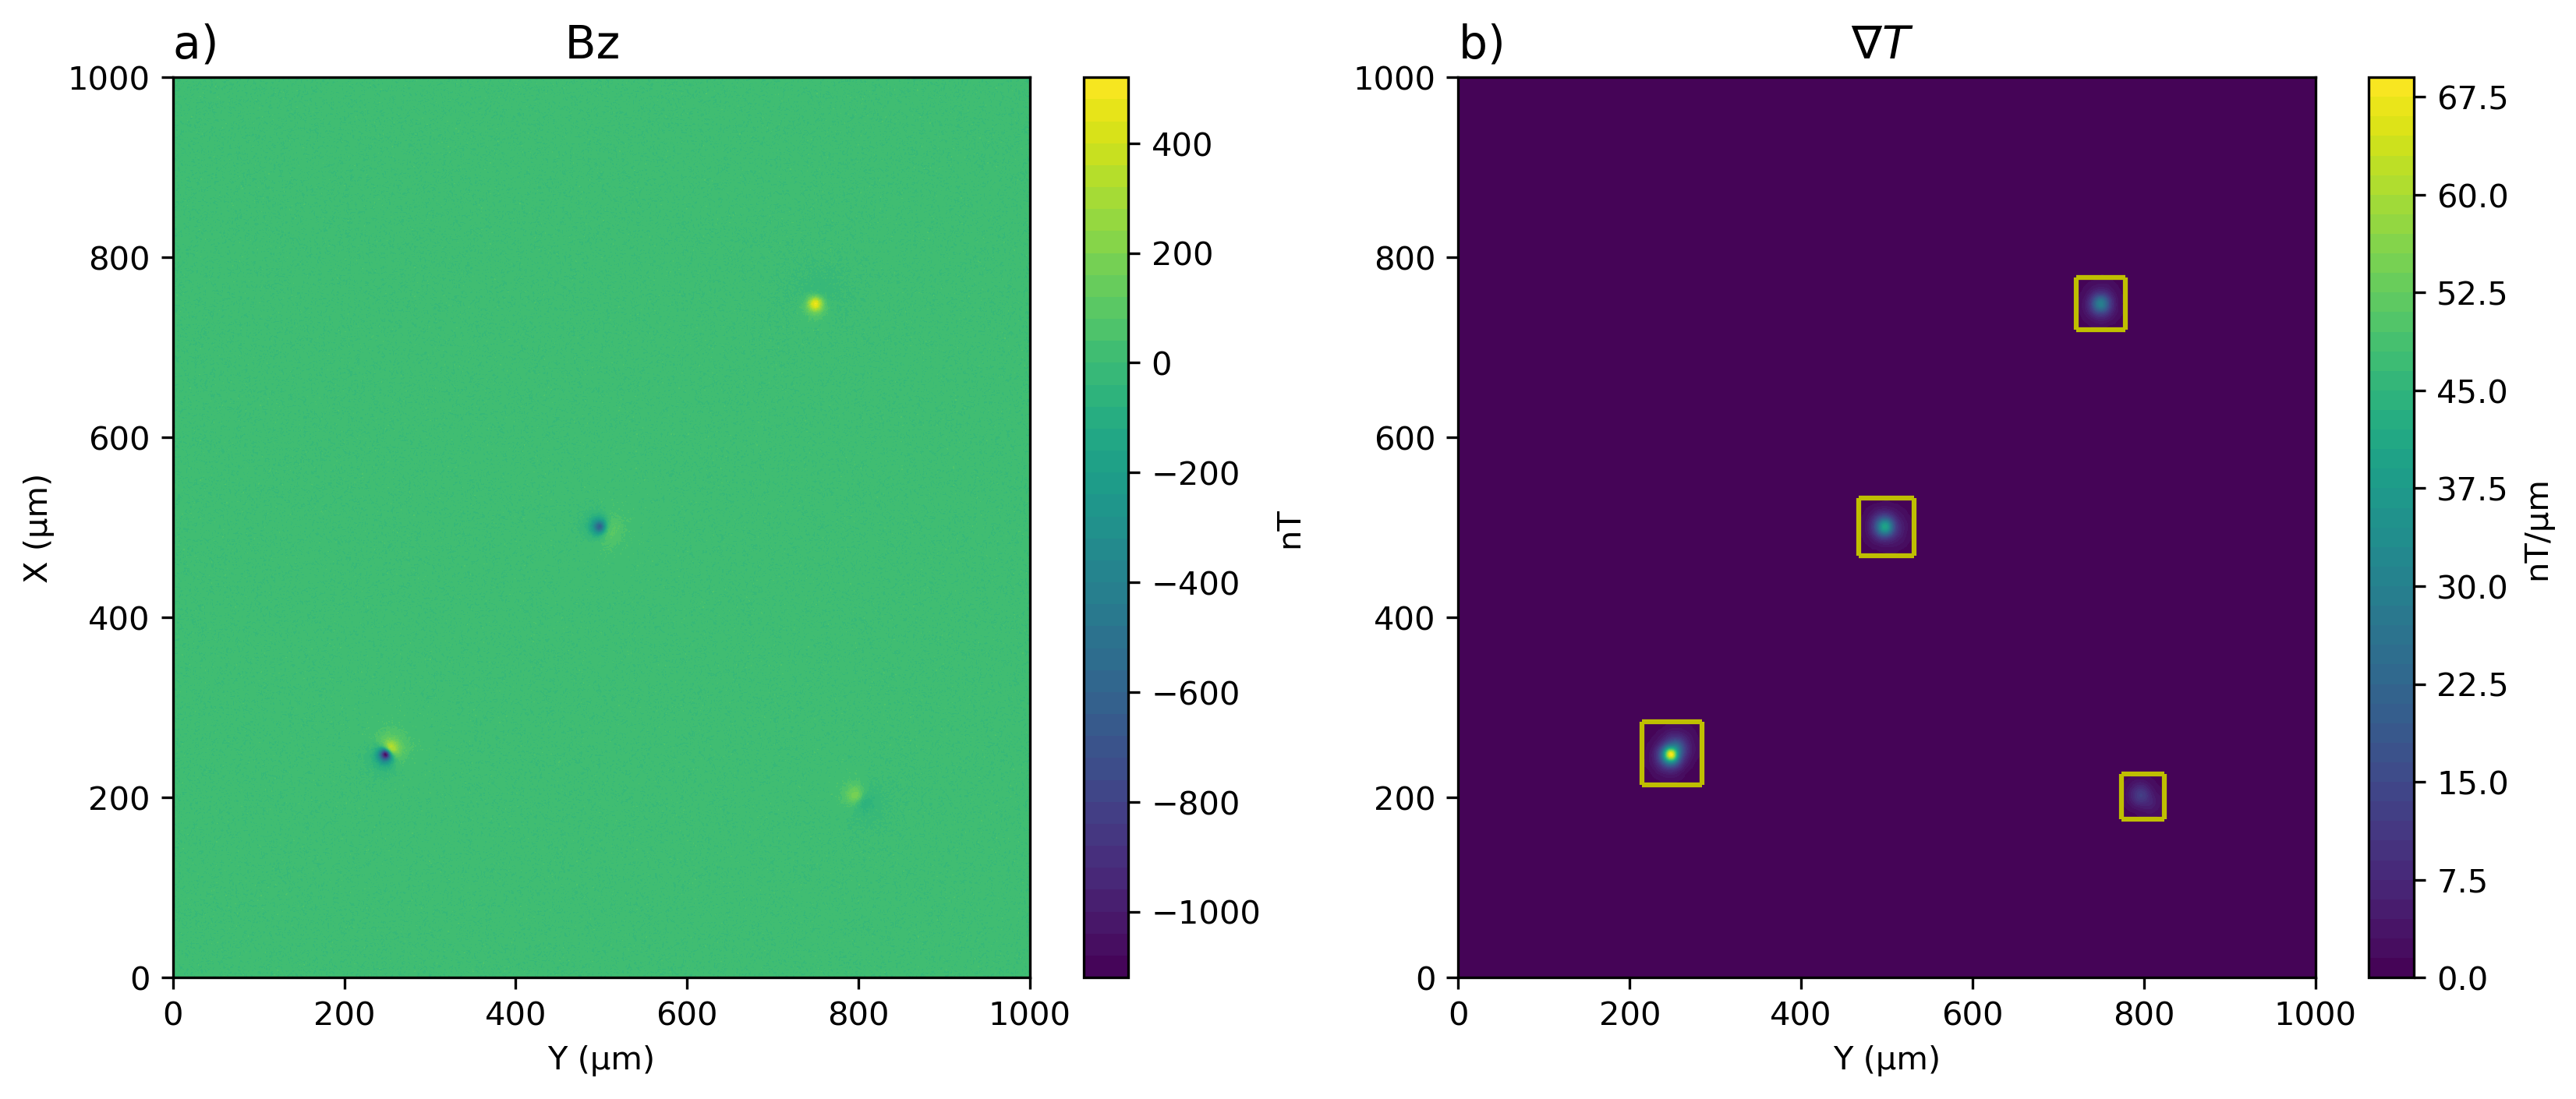
\includegraphics[width=1.0\textwidth]{SimpleSynthetic.png}
\caption{a) Synthetic data contaminated with psedo-random normal noise. b) Individual sources window position (yellow squares) obtained with the blob detection algorithm applied on the total gradient map.}
\label{fig:SimpleSynthetic}
\end{figure}

\bigskip

\noindent{After isolante the potencial field data and first derivatives for each source, we can solve the 3D Euler deconvolution \cref{eq:euler2} proposed by  \cite{Reid1990}, one for each subarea selected (window data), by assuming the structural index of a sphere/punctual source (N = 3). Thus, obtaining a sturdy result for the central positioning (Xc, Yc, Zc) of each source causing the magnetic potential anomaly in the observed data set, as shown in \cref{tab:InversionTab}.}

\noindent{The last step consists of using the central positions of each source, obtained with Euler's method, as an input parameter for inverting the original noisy data (\cref{fig:SimpleSynthetic}a) to find the least squares (or robust) approximation solution for the vector of cartesian magnetic moments ($\bar{m}$). With this, the magnetization directions (D and I) and the intensity of the magnetic moment can be estimated using equations (\cref{eq:sphere16,eq:sphere17,eq:sphere17_m}), as well as the uncertainty propagation of this inversion, using equations (\cref{eq:sphere21,eq:sphere22,eq:sphere22_m}) and considering $\sigma$ = 25nT. The results obtained with the least squares estimator can also be seen in \cref{tab:InversionTab}.}

\bigskip

% If you use beamer only pass "xcolor=table" option, i.e. \documentclass[xcolor=table]{beamer}

\begin{table}[htbp]
\caption{Positioning and magnetization parameters recovered with the inversion.}
\label{tab:InversionTab}
\resizebox{1.0\textwidth}{!}{
\begin{tabular}{ccccccc}
\hline   
\rowcolor[HTML]{FFFFFF} 
\cellcolor[HTML]{FFFFFF}                         & \multicolumn{3}{c}{\cellcolor[HTML]{FFFFFF}Center coordinates}                    & \multicolumn{3}{c}{\cellcolor[HTML]{FFFFFF}Magnetization}     \\
\rowcolor[HTML]{FFFFFF} 
\multirow{-2}{*}{\cellcolor[HTML]{FFFFFF}Sphere} & Xc ($\mu m$) & Yc ($\mu m$) & Zc ($\mu m$) & m ($A \cdot m^2$) & D (\textdegree) & I (\textdegree) \\  \hline   
1                                                & 250.28           & 250.19           & 5.38           & 8.82e-15  $\pm$  1.39e-17           & -140.22  $\pm$  0.11           & -30.04  $\pm$  0.08           \\
\rowcolor[HTML]{FFFFFF} 
2                                                & 500.46           & 500.50           & 7.77           & 7.67e-15  $\pm$  1.90e-17           & -69.42  $\pm$  0.26           & -49.85  $\pm$  0.15           \\
3                                                & 750.73           & 750.72           & 8.57           & 6.31e-15  $\pm$  1.99e-17           & 9.06  $\pm$  0.50           & 62.34  $\pm$  0.22           \\
\rowcolor[HTML]{FFFFFF} 
4                                                & 200.30           & 800.92           & 10.00           & 4.94e-15  $\pm$  3.01e-17           & 124.63  $\pm$  0.39           & 21.76  $\pm$  0.27           \\ \hline                 
\end{tabular}
}
\end{table}



\noindent{It is important to emphasize that \cite{OliveiraJr.2015} proved that the magnetization directions (D and I) recovered by the least squares estimator is sensitive to variations in the horizontal coordinates (x and y) of the magnetic sources central positions. While, the same being practically insensitive to variations in depths. Thus, the same authors consider Euler deconvolution method as an adequate technique to estimate the central positions that will be used as a priori information for inversion. This occurs mainly because, when well performed, the recovery of the horizontal coordinates of sources central position is considerably accurate, while the vertical coordinate can undergo greater variation \citep{Silva2003, Melo2013}, even so the inversion will still provide extremely satisfactory results. The high sensitivity of Euler deconvolution to high frequency noise can also be easily overcome with the proper application of the upward continuation filter.}



\subsection{Complex Simulation: Testing Applicability}



\section{Aplication to Real Data}

\section{Discussion}

\begin{singlespace}

\section{Conclusion}

\noindent{We developed an efficient semi-automated method to determine the direction of magnetization of dipolar sources on a microscale, as well as the recovery of their magnetic moment. Being ideal for a reinterpretation for the application of methods of paleomagnetic studies using thin sections of rock samples. This would be an attempt to improve the quality of results obtained by isolating the responses of more reliable recorders of the Earth's geomagnetic field. }

\noindent{We also present a new, faster and cleaner way to solve the Euler equation in determining the positioning of magnetic anomaly sources using a pre-selection of magnetic anomaly source windows based on the Laplacian of the Gaussian applied to total gradient anomaly maps. In this way, reducing the numerous solutions to just one data window per source. After estimating the structural index (N = 3) by approximating the sources generating the magnetic anomaly to spheres/points, the Euler deconvolution is performed and the central position of each source is determined.}

\noindent{Since for the recovery of direction and magnetization we only need to assume that the sources have their central positions known (so we apply Euler deconvolution) and that their magnetizations are uniform. This last premise aligns with the theory of magnetically stable particles, which are the basis of classical paleomagnetism. Also, there is no need for any kind of prior knowledge other than the observed magnetic anomaly, and the structural index of the sources. Therefore, this method can be quickly replicated in a dataset of thin sections of rocks to obtain the distributions of magnetic directions of each source identified in the sample.}

\noindent{The test using a simply synthetic sample shows the great capability of the method by retrieving not only the precisely center positions }


\end{singlespace}

\begin{singlespace}
\doublespacing
\bibliographystyle{agu}  % style file is seg.bst
\bibliography{article1}
\end{singlespace}


\newpage

\section{Appendix A}
\subsection{Appendix A.1}
\label{AppendixA1}

\noindent{As the least squares estimate (\cref{eq:sphere11}) is very sensitive to the presence of outliers in the observed data, the estimated parameters could be seriously misleading. To counteract this problem \cite{OliveiraJr.2015} suggest a robust scheme based on the minimization of the objective function obtained with the absolute error:}

\begin{equation} \label{eq:sphere12}
\centering
\small f\left(\widetilde{m}\right)=\left(\sum_{i=1}^{N}\left| { \left(\bar{\bar{A}} \cdot \bar{m} \right)}_{i} - {{\bar{\left(B_z\right)}}}_{i} \right|\right)
\end{equation}

\noindent{Unlike the solution presented for the objective function in \cref{eq:sphere11}, the parameter vector minimizing \cref{eq:sphere12} cannot be obtained as a simple linear system. A practical way is the iteratively reweighted least squares algorithm \citep{Aster2019, OliveiraJr.2015}. In this algorithm, at each iteration k, the following linear system is solved:}

\begin{equation} \label{eq:sphere13}
\centering
\small {\widetilde{m}}^{k+1}=\left({\bar{\bar{A}}}^T\cdot{\bar{\bar{R}}}^k\cdot\bar{\bar{A}}\right)^{-1}\cdot\left({\bar{\bar{A}}}^T\cdot{\bar{\bar{R}}}^k\cdot{\bar{B}}_z\right)\ \ 
\end{equation}

\noindent{The term ${\bar{\bar{R}}}^k$ is an N $\times$ N diagonal matrix whose i-th element $r_i^k$ (i = 1, 2, ..., N) is given by:}

\begin{equation} \label{eq:sphere14}
{r_i}^k=\frac{1}{\left|\left(\bar{\bar{A}}\cdot\bar{m}\right)_i-{{\bar{B_z}}}_i+e\right|}
\end{equation}

\begin{FlushRight}
\noindent{Where: $e$ is a small positive number used to prevent singularities}
\end{FlushRight}

\noindent{This iterative process starts (k = 0) with the solution vector obtained by the least squares estimator (\cref{eq:sphere11}). From this initial approximation ${\widetilde{m}}^0$, we calculate the matrix ${\bar{\bar{R}}}^0$ (\cref{eq:sphere14}). Which is used in the solution of the linear system given by \cref{eq:sphere13} to obtain the estimate ${\widetilde{m}}^1$. Later using this updated estimate to calculate the new matrix ${\bar{\bar{R}}}^1$ (\cref{eq:sphere14}), we solve the linear system (\cref{eq:sphere13}) to obtain a new estimate ${\widetilde{m}}^ 2$, and so on. As the iterations progress, this iterative procedure tends to converge and estimate $\widetilde{m}$, which is called robust estimate \citep{OliveiraJr.2015}. According to \cite{Aster2019} this convergence can be limited by a tolerance $\tau$, given by:}

\begin{equation} \label{eq:sphere15}
\centering
\frac{\lVert {\widetilde{m}}^{k+1} - {\widetilde{m}}^{k} \lVert}{1 + \lVert \widetilde{m}^{k+1} \lVert} ≤ \tau
\end{equation}

\begin{FlushRight}
\noindent{Where: $\tau$ is a positive number (\emph{e.g.}, ${10}^{-2}$) chosen by the algorithm user.}
\end{FlushRight}

\noindent{The convariance matrix for the uncertainties propagation also is updated with the ${\bar{\bar{R}}}^k$, as shown in the \cref{eq:sphere19}:}

\begin{equation} \label{eq:sphere19}
\centering
\small \bar{\bar{Cov}}\left(\widetilde{m_j}\right)=\ {\sigma_0}^2\cdot\left({\bar{\bar{A}}}^T\cdot ~ {\bar{\bar{R}}}^k\cdot ~ \bar{\bar{A}}\right)^{-1} \ \ \text{(\emph{robust})}
\end{equation}


\subsection{Appendix A.2} 
\label{AppendixA2}

\noindent{The derivatives of the propagation functions of the uncertainties of the declination ($\sigma_{D_j}$), inclination ($\sigma_{I_j}$) and magnetic moment ($\sigma_{m_j}$) in relation to each parameter ($mx_j, my_j, mz_j$) are detailed below:}

\begin{equation} \label{eq:sphere23}
\centering
\frac{\partial D_j}{\partial{mx}_j}=\frac{-{my}_j}{{{mx}_j}^2+{{my}_j}^2}
\end{equation}

\begin{equation} \label{eq:sphere24}
\centering
\frac{\partial D_j}{\partial{my}_j}=\frac{{mx}_j}{{{mx}_j}^2+{{my}_j}^2}
\end{equation}

\begin{equation} \label{eq:sphere25}
\centering
\frac{\partial I_j}{\partial{mx}_j}=\frac{-{mx}_j\cdot \ {mz}_j}{\sqrt{{{mx}_j}^2+{{my}_j}^2}\cdot \left({{mx}_j}^2+{{my}_j}^2+{{mz}_j}^2\right)}
\end{equation}

\begin{equation} \label{eq:sphere26}
\centering
\frac{\partial I_j}{\partial{my}_j}=\frac{-{my}_j\cdot \ {mz}_j}{\sqrt{{{mx}_j}^2+{{my}_j}^2}\cdot \left({{mx}_j}^2+{{my}_j}^2+{{mz}_j}^2\right)}
\end{equation}

\begin{equation} \label{eq:sphere27}
\centering
\frac{\partial I_j}{\partial{mz}_j}=\frac{\sqrt{{{mx}_j}^2+{{my}_j}^2}}{\left({{mx}_j}^2+{{my}_j}^2+{{mz}_j}^2\right)}
\end{equation}

\begin{equation} \label{eq:sphere28}
\centering
\frac{\partial m_j}{\partial{mx}_j}=\frac{{mx}_j}{ \sqrt{{{mx}_j}^2+{{my}_j}^2+{{mz}_j}^2} }
\end{equation}

\begin{equation} \label{eq:sphere29}
\centering
\frac{\partial m_j}{\partial{my}_j}=\frac{{my}_j}{ \sqrt{{{mx}_j}^2+{{my}_j}^2+{{mz}_j}^2} }
\end{equation}

\begin{equation} \label{eq:sphere30}
\centering
\frac{\partial m_j}{\partial{mz}_j}=\frac{{mz}_j}{ \sqrt{{{mx}_j}^2+{{my}_j}^2+{{mz}_j}^2} }
\end{equation}


\end{document}
